% Requires graphicx. Copy the accompanying figures directory.
\begin{figure}[t]\centering
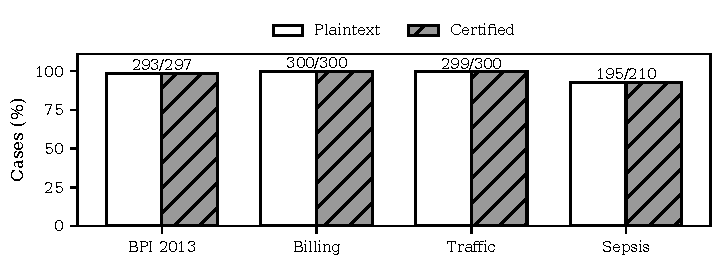
\includegraphics[width=\linewidth]{figures/fig_utility.pdf}
\caption{Threshold agreement at $K=1$ on the four frozen held-out cohorts. Plaintext bars count cases whose reference alignment cost is at most the threshold. Certified bars count distinct cases accepted by the auditor using actual proofs. The denominator includes every case in each cohort.}
\label{fig:eval-utility}
\end{figure}
\begin{figure}[t]\centering
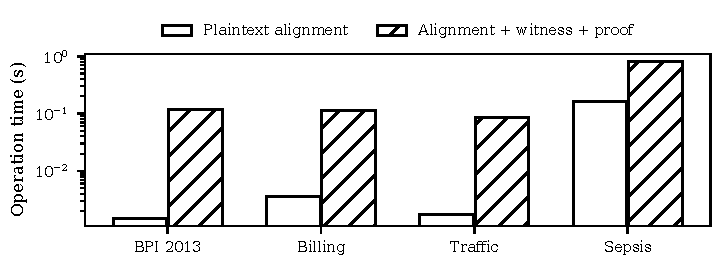
\includegraphics[width=\linewidth]{figures/fig_overhead.pdf}
\caption{Mean operation time on selected short, median, and long alignments, with five repetitions per selected case. The protected computation includes plaintext alignment, witness encoding, and proving. Setup and artifact loading are excluded from these operation times and recorded separately.}
\label{fig:eval-overhead}
\end{figure}
\begin{figure}[t]\centering
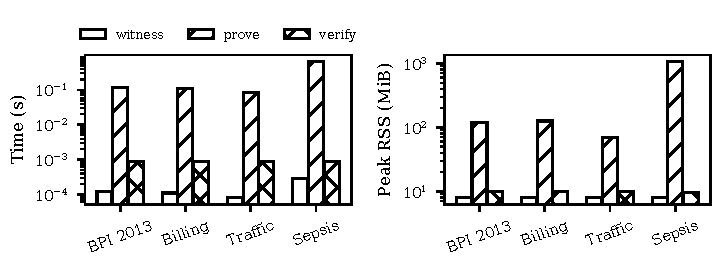
\includegraphics[width=\linewidth]{figures/fig_time_memory.pdf}
\caption{Mean operation time and mean per-process peak resident memory for witness encoding, proving, and verification on the selected cases. Each stage and repetition runs in a fresh process. Process peaks include loaded artifacts and serialization. Proving includes constraint solving.}
\label{fig:eval-time_memory}
\end{figure}
\begin{figure}[t]\centering
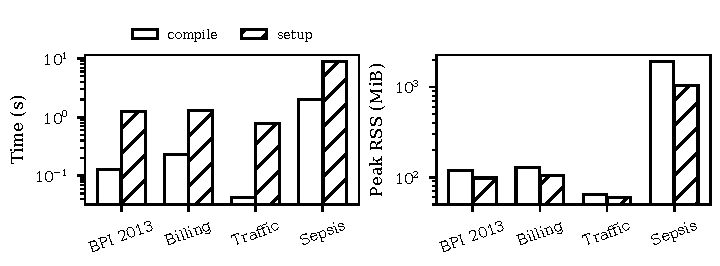
\includegraphics[width=\linewidth]{figures/fig_setup_time_memory.pdf}
\caption{Compilation and setup measured independently in fresh processes, with five repetitions per model. Time refers to the named operation, while resident memory is the peak of the complete worker process.}
\label{fig:eval-setup_time_memory}
\end{figure}
\begin{figure}[t]\centering
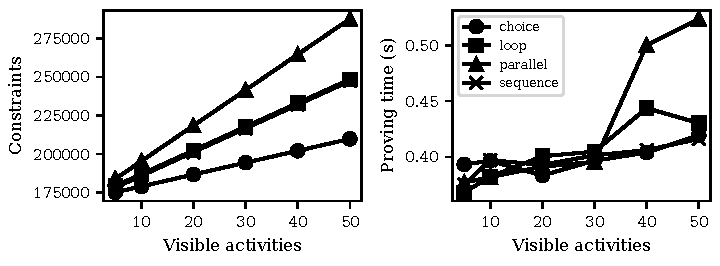
\includegraphics[width=\linewidth]{figures/fig_model_scalability.pdf}
\caption{Controlled model scaling for sequence, choice, parallel, and loop structures. Trace capacity is 128 and alignment capacity is 256 for every model. Proving times average three repetitions per model.}
\label{fig:eval-model_scalability}
\end{figure}
\begin{figure}[t]\centering
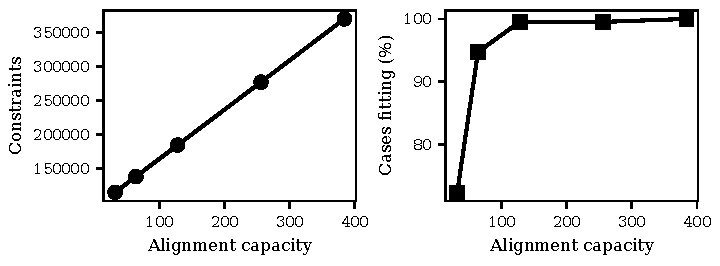
\includegraphics[width=\linewidth]{figures/fig_capacity.pdf}
\caption{Effect of alignment capacity for the fixed Sepsis model and a trace capacity of 185. Coverage counts all held-out traces whose reference alignment fits, regardless of whether its cost meets the audit threshold.}
\label{fig:eval-capacity}
\end{figure}
\begin{figure}[t]\centering
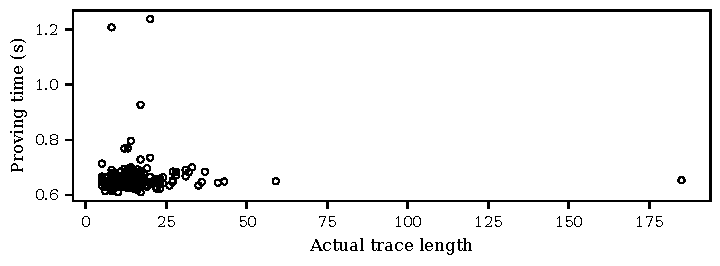
\includegraphics[width=\linewidth]{figures/fig_trace_length.pdf}
\caption{Observed proving times for certified Sepsis traces at fixed capacities. These are observations from the functional cohort run, not the dedicated repeated performance sample.}
\label{fig:eval-trace_length}
\end{figure}
\begin{figure}[t]\centering
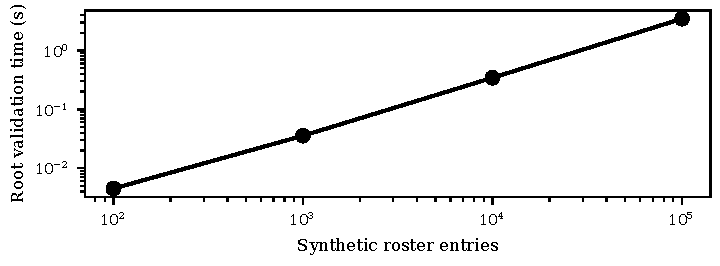
\includegraphics[width=\linewidth]{figures/fig_population.pdf}
\caption{Fresh-process root validation for synthetic rosters of distinct commitments. This experiment measures population-root checking, not verification of an equal number of proofs. Separate experiments verify distinct real certificates for populations of 100 and 300 cases.}
\label{fig:eval-population}
\end{figure}
